\chapter{Wat is bitcoin?}

Bitcoin is een vorm van \textit{peer-to-peer elektronisch geld}, een nieuwe vorm van digitaal geld dat kan worden overgedragen tussen mensen of computers zonder enige vertrouwde tussenpersoon (zoals een bank), en waarvan de uitgifte niet gecontroleerd wordt door één enkele partij. 

Denk aan een papieren dollar of fysieke, metalen munt. Wanneer je die aan anderen geeft, hoeven ze niet te weten wie je bent. Zij moeten er alleen op te vertrouwen dat het geld dat ze van je krijgen geen vervalsing is. Normaal gesproken vertrouwen mensen bij fysiek geld op hun ogen en vingers, of bij grotere hoeveelheden op het gebruik van testapparatuur om vals van echt te onderscheiden.

Maar in de digitale samenleving worden de meeste van onze betalingen gedaan via een tussenpersoon: via een bank met behulp van IDeal, een kredietkaartmaatschappij zoals Visa, een digitale betalingsprovider zoals PayPal, of WeChat in China.

Met de overgang naar de digitale wereld is geld veranderd van een fysiek iets dat je zelf kunt bijhouden, overdragen en verifiëren, naar digitale bits die door een derde partij worden opgeslagen, geverifieerd en verstuurd. Daardoor ben je voor elke digitale financiële handeling nu afhankelijk van een derde partij. 

Omdat we ons contant geld opgeven voor het gemak van digitale betalingen, creëren we ook een systeem waarin anderen buitengewone macht hebben om ons te onderdrukken. Digitale betalingsplatformen zijn de basis geworden van dystopische, autoritaire controlesystemen die bijvoorbeeld worden gebruikt door de Chinese overheid om afvalligen te controleren en om te voorkomen dat specifieke burgers goederen of diensten gebruiken. 

Bitcoin biedt een alternatief voor centraal gestuurd, digitaal geld. Het biedt os een systeem dat ons de vrijheid van contant geld teruggeeft, maar op digitale wijze: 

\begin{enumerate}
    \item Een digitaal bezit waarvan het aanbod beperkt, vooraf bekend en onveranderlijk is. Dit staat in schril contrast met bankbiljetten en hun digitale versies die worden uitgegeven door overheden en centrale banken, waarvan het aantal zich in een onvoorspelbaar tempo blijft uitbreiden.
    \item Een stel onderling verbonden computers (\textit{het bitcoinnetwerk}), waar iedereen kan aan deelnemen door een stukje software te draaien op hun computer. Dit netwerk dient om bitcoins uit te geven, hun eigendomstitel te volgen en om overdrachten tussen deelnemers uit te voeren, zonder te vertrouwen op tussenpersonen zoals banken, betalingsbedrijven en overheidsinstanties.
    \item De bitcoinclientsoftware, een stukje computercode die iedereen kan uitvoeren om deelnemer te worden van het netwerk. Deze software is \textit{open source}, wat betekent dat iedereen kan zien hoe het werkt en bij kan dragen aan nieuwe functies en verbeteringen.

\end{enumerate}
\begin{figure}
    \centering
    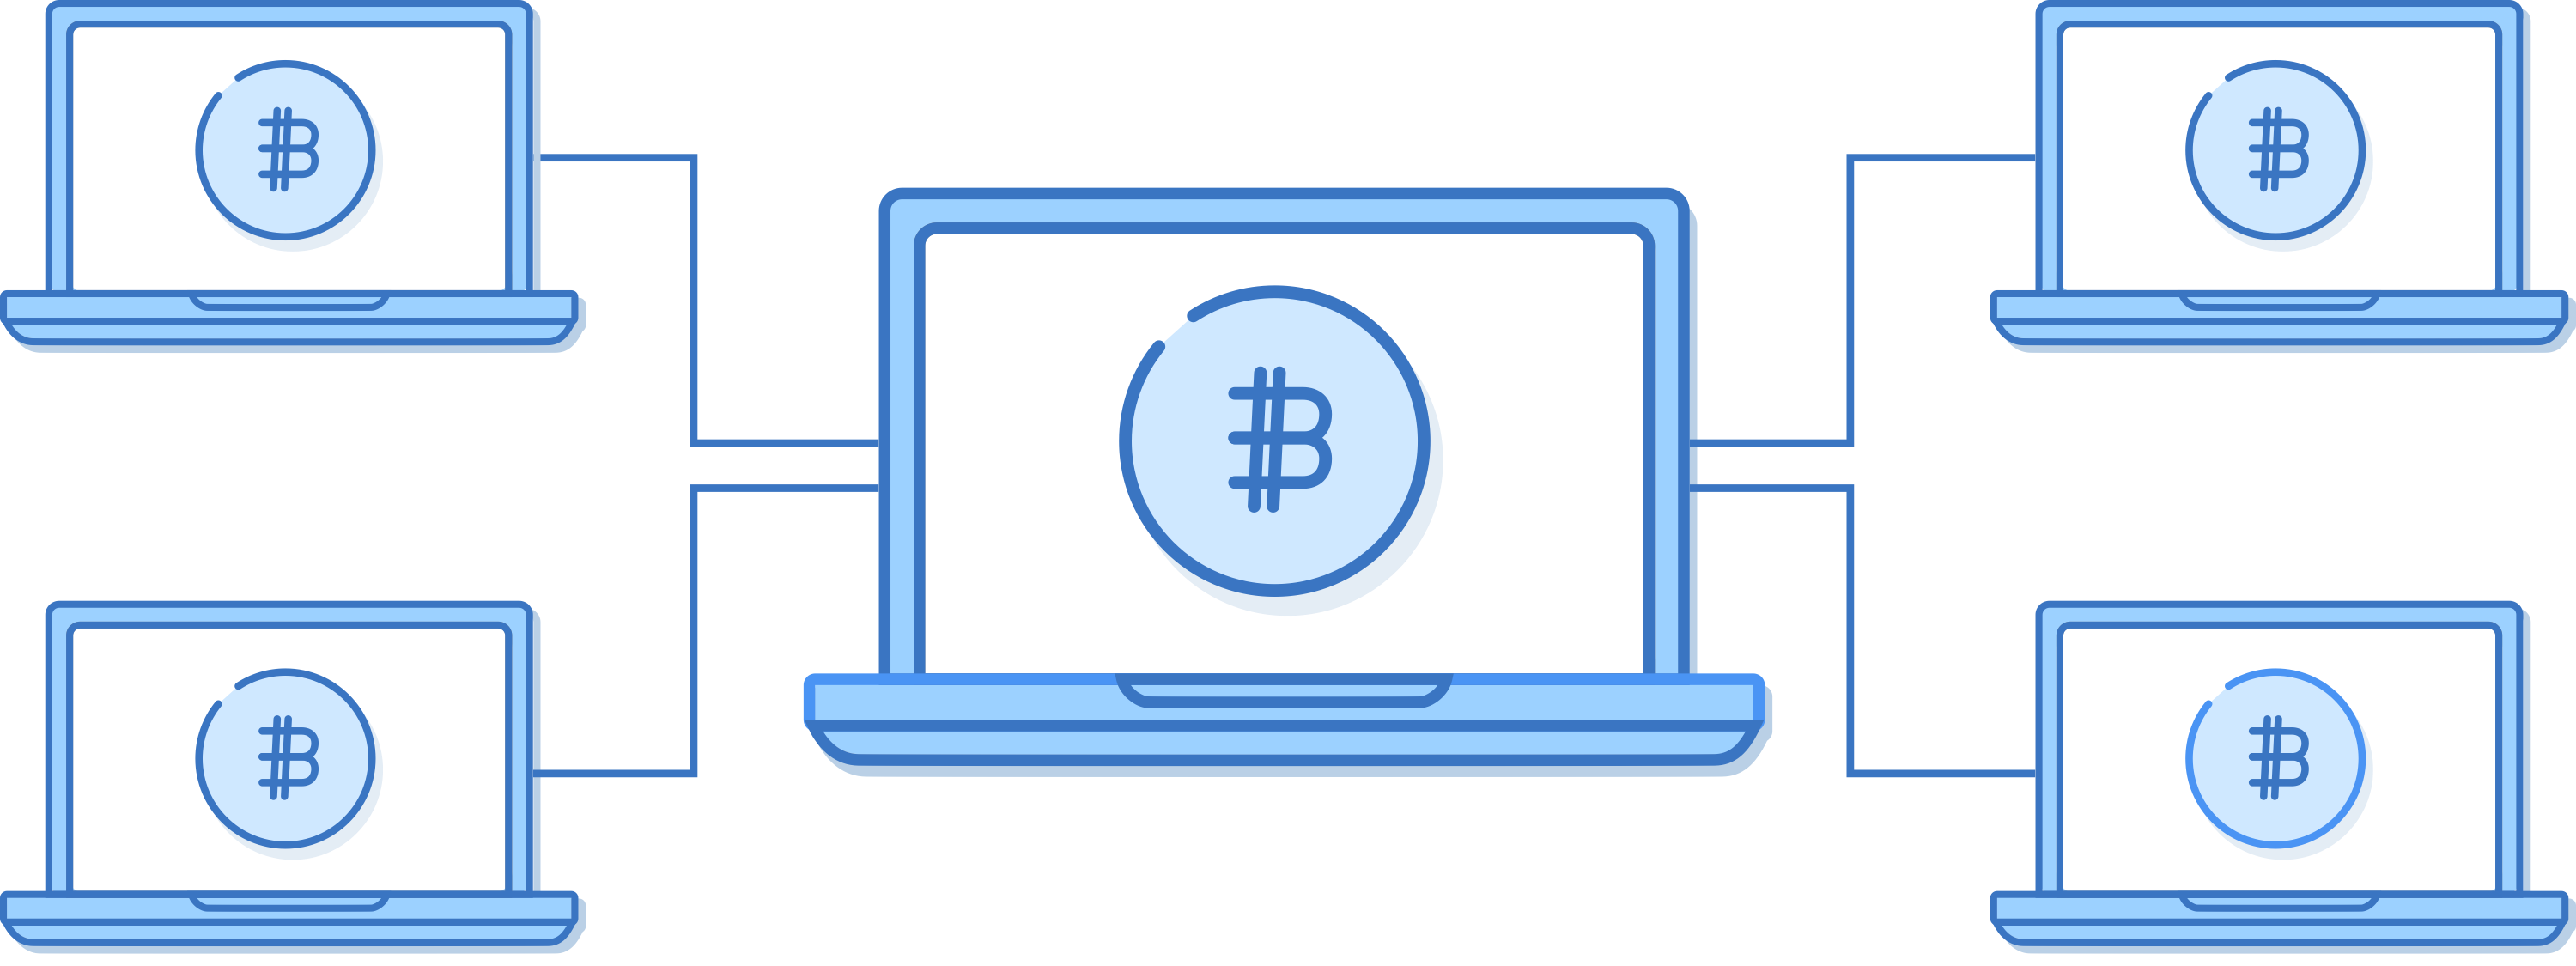
\includegraphics[width=\textwidth]{images/fig1.png}
    \caption{\footnotesize{\textit{Bitcoin is een netwerk van computers die de bitcoinclientsoftware draaien}.}}
    \label{fig1}
\end{figure}

\noindent Later in het boek komen we terug op de motivaties achter bitcoin.

\section{Waar komt bitcoin vandaan?}

Bitcoin is rond 2008 uitgevonden door een of meer personen die bekend staan onder het pseudoniem  \href{https://nl.wikipedia.org/wiki/Satoshi_Nakamoto}{\textbf{Satoshi Nakamoto}}\footnote{Door de gemeenschap wordt gerefereerd aan Satoshi als man. In dit boek zullen we ook als dusdanig naar hem refereren ondanks dat het onbekend is of het gaat om een man, vrouw of groep personen}. Niemand kent de identiteit van Satoshi, en voor zover we weten is hij verdwenen en heeft hij al jaren niets meer van zich laten horen.

Op 11 februari 2009 berichtte Satoshi over een vroege versie van bitcoin op een online forum voor mensen die werken aan cryptografie en veel waarde hechten aan individuele privacy en vrijheid --- \textit{cypherpunks}. Hoewel dit niet de eerste officiële aankondiging van bitcoin was, bevatte het een goede samenvatting van Satoshi's beweegredenen. Daarom gebruik ik het om de basis te leggen voor onze discussie.

Ik zal een aantal citaten weergeven die verduidelijken welke problemen van het huidige financiële systeem Satoshi probeerde op te lossen:

\begin{quotation}
Ik heb een nieuw open source P2P e-cash systeem ontwikkeld genaamd bitcoin. Het is volledig gedecentraliseerd, zonder centrale server of vertrouwde partijen. Alles is gebaseerd op cryptografisch bewijs in plaats van vertrouwen. [...]

Het kernprobleem met conventionele valuta is het vertrouwen dat nodig is om het te laten werken. De centrale bank moet worden vertrouwd, maar de geschiedenis van fiatvaluta zit vol met schendingen van dat vertrouwen. We moeten banken vertrouwen om ons geld te bewaren en elektronisch over te maken, maar ze lenen het uit in golven van kredietbubbels met nauwelijks een fractie van die waarde in reserve. We moeten hen onze privacy toevertrouwen, en we moeten erop vertrouwen dat ze identiteitsdieven weerhouden om onze rekeningen te plunderen. Hun enorme overheadkosten maken microbetalingen onmogelijk.

Vroeger hadden \textquotedbl{}multi-user time-sharing computersystemen\textquotedbl{} een vergelijkbaar probleem. Voor sterke encryptie moesten gebruikers nog vertrouwen op wachtwoorden om hun bestanden te beveiligen [...]

Toen werd sterke encryptie beschikbaar voor de massa en was vertrouwen niet langer nodig. Gegevens konden worden beveiligd waardoor het voor anderen onmogelijk was om toegang te krijgen, ongeacht om welke reden, ongeacht hoe goed het excuus, wat er ook gebeurt.

Het wordt tijd dat we dit ook hebben voor geld. Met e-valuta op basis van cryptografisch bewijs, zonder de noodzaak om een externe tussenpersoon te vertrouwen. Geld kan veilig zijn en transacties moeiteloos. [...]

De oplossing van bitcoin is om een peer-to-peer-netwerk te gebruiken om te controleren op dubbele uitgaven. In een notendop werkt het netwerk als een gedistribueerde tijdstempel, waarbij de eerste uitgave van een munt van een tijdstempel wordt voorzien. Het maakt gebruik van het feit dat informatie gemakkelijk te verspreiden is, maar moeilijk is om tegen te houden.

Voor meer informatie over hoe het werkt, zie het ontwerpdocument op \href{http://www.bitcoin.org/bitcoin.pdf}{http://www.bitcoin.org/bitcoin.pdf}.\footnote{Kijk voor de Nederlandse versie van de whitepaper op: \href{https://btcdirect.eu/nl-nl/bitcoin-whitepaper}{https://btcdirect.eu/nl-nl/bitcoin-whitepaper}}
\par\raggedleft--- \textup{SATOSHI NAKAMOTO}
\end{quotation}

\section{Welke problemen lost het op?}

Laten we een aantal van Satoshi's beweringen nader onderzoeken. Doorheen het boek zullen we bespreken hoe deze concepten daadwerkelijk worden geïmplementeerd. Maak je geen zorgen als iets onbekend aanvoelt in deze sectie want we gaan er later dieper op in. Het idee is om de bedoeling van Satoshi te begrijpen, zodat we ze later in dit boek kunnen onderzoeken.

\begin{quote}
\textit{Ik heb een nieuw open source P2P e-cash systeem ontwikkeld}
\end{quote}

P2P staat voor \textit{peer-to-peer} en geeft een systeem aan waarbij één persoon een interactie heeft met een ander, zonder tussenpartij. De twee partijen (ontvanger en verzender) zijn gelijkwaardig. Je herinnert je misschien P2P-technologieën zoals Napster, Kazaa en BitTorrent, waarmee mensen voor het eerst met elkaar bestanden, muziek en films konden delen zonder tussenpersoon. Satoshi ontwierp bitcoin om mensen de mogelijkheid te geven om op vrijwel dezelfde manier elektronisch contant geld (\textit{e-cash}) uit te wisselen zonder tussenpersoon.

De software is \textit{open source}, wat betekent dat iedereen kan zien hoe het werkt en iedereen kan bijdragen. Dit is belangrijk omdat het zorgt voor transparantie. Er is geen vertrouwen nodig. We hoeven niets te geloven van wat Satoshi schreef in zijn berichten over hoe de software werkt. We kunnen de code bekijken en controleren hoe het werkt. Bovendien kunnen we de functionaliteit van het systeem verbeteren door de code te wijzigen.

\begin{quote}
\textit{Het is volledig gedecentraliseerd, zonder centrale server of vertrouwde partijen...}
\end{quote}

Satoshi vermeldt dat het systeem \textit{gedecentraliseerd} is om het te onderscheiden van systemen die wel centrale aansturing hebben. Eerdere pogingen om digitaal contant geld te creëren, zoals DigiCash van David Chaum, werden ondersteund door een \textit{centrale server}; een computer of set van computers die verantwoordelijk waren voor uitgifte en verificatie van betalingen, onder controle van één bedrijf.

Dergelijke centraal aangestuurde particuliere vormen van digitaal geld zijn gedoemd te mislukken; we kunnen niet vertrouwen op geld dat kan verdwijnen wanneer een bedrijf failliet gaat, wordt gehackt, last heeft van IT-problemen of wordt gestopt door de overheid.

Bitcoin, aan de andere kant, wordt niet gerund en gecontroleerd door een enkel bedrijf, maar door een netwerk van individuen en bedrijven van over de hele wereld. Het stoppen van bitcoin vereist het stoppen van tienduizenden tot honderdduizenden computers over de hele wereld, waarvan velen lastig te traceren zijn. Het is een hopeloos kat-en-muisspel aangezien elke aanval van deze aard eenvoudigweg de creatie van nieuwe \textit{bitcoin-nodes} of computers op het netwerk aanmoedigt.

\begin{quote}
\textit{ ... alles is gebaseerd op cryptografisch bewijs in plaats van vertrouwen}
\end{quote}

Het internet en de meeste moderne computersystemen zijn gebouwd op cryptografie; een methode om informatie te versleutelen zodat alleen de ontvanger van de informatie deze kan ontcijferen. Hoe ontsnapt bitcoin aan de noodzaak van \textit{vertrouwen}? We zullen hier later in het boek op ingaan, maar het basisidee is dat in plaats van iemand te vertrouwen die zegt \textquotedbl{}Ik ben Alice\textquotedbl{} of \textquotedbl{}Ik heb \$10 in mijn account\textquotedbl{}, we cryptografie kunnen gebruiken om dezelfde feiten dusdanig te presenteren zodat de ontvanger van het bericht dit eenvoudig zelf kan verifiëren en het onmogelijk is om te vervalsen. Bitcoin maakt gebruik van cryptografie om deelnemers in staat te stellen het gedrag van alle anderen te controleren, zonder dat hierbij een centrale partij vertrouwt hoeft te worden.

\begin{quote}
\textit{We moeten hen [de banken] onze privacy toevertrouwen, en we moeten erop vertrouwen dat ze identiteitsdieven ervan weerhouden om onze rekeningen te plunderen}
\end{quote}

In tegenstelling tot het gebruik van een bankrekening, het digitale betalingssysteem of kredietkaarten, stelt bitcoin twee partijen in staat om transacties uit te voeren zonder persoonlijke identificatie op te geven. Banken, kredietkaartmaatschappijen, betalingsverwerkers en overheden beschikken over gecentraliseerde databanken van consumentengegevens. Deze gegevens zijn een gigantische buit voor hackers. Zo werden bij de hack van Equifax in 2017 de identiteits- en financiële gegevens van meer dan 140 miljoen mensen buitgemaakt. Dit soort databanken en de bijbehorende hacks kunnen resulteren in identiteitsfraude op grote schaal. 

Bitcoin ontkoppelt financiële transacties van identiteiten uit de echte wereld. Immers, wanneer we contant geld aan iemand geven, hoeft de ontvanger niet te weten wie we zijn en hoeft de betaler zich geen zorgen te maken dat zijn informatie wordt gebruikt om hem op een later moment te bestelen. Waarom zouden we niet hetzelfde, of meer, verwachten van digitaal geld?

\begin{quote}
\textit{De centrale bank moet worden vertrouwd om de valuta niet te devalueren, maar de geschiedenis van fiatvaluta zit vol met schendingen van dat vertrouwen}
\end{quote}

\textit{Fiat}, Latijn voor \textquotedbl{}laat het gebeuren\textquotedbl{}, verwijst naar valuta uitgegeven door de overheid en centrale bank en dat door de overheid als wettig betaalmiddel is aangenomen. Historisch gezien werd geld gemaakt uit dingen die moeilijk zijn om te produceren, gemakkelijk zijn om te verifiëren en gemakkelijk zijn om te vervoeren, zoals schelpen, glaskralen, zilver en goud. Telkens wanneer iets als geld werd gebruikt, bestond de verleiding om er meer van te maken. Als iemand langskwam met superieure technologie om snel veel van iets te creëren, verloor het goed zijn waarde. Zo konden Europese kolonisten het Afrikaans continent ontdoen van haar rijkdom, door te handelen in glazen kralen die voor de Europeanen gemakkelijk, maar voor de Afrikanen moeilijk, te produceren waren. Dit is waarom goud al zo lang wordt beschouwd als betrouwbare vorm van geld - het is moeilijk om snel meer goud te produceren.\footnote{Voor een goed overzicht van de monetaire geschiedenis raad ik het essay \textit{Shelling Out} van Nick Szabo aan: \href{https://nakamotoinstitute.org/shelling-out}{https://nakamotoinstitute.org/shelling-out}}

We zijn langzaam overgestapt van een wereldeconomie met goud als geld naar een wereld waarbij papieren certificaten werden uitgegeven als claim op datzelfde goud. Uiteindelijk werden door president Nixon de papieren claims volledig losgekoppeld van goud. Hij maakte in 1971 een einde aan de internationale inwisselbaarheid van de Amerikaanse dollar voor goud.

Het einde van de goudstandaard stelde overheden en centrale banken in staat om de geldhoeveelheid naar believen te vergroten, waardoor ieder biljet in omloop minder waard werd. Dit staat bekend als \textit{geldontwaarding}. Hoewel fiatvaluta wordt uitgegeven door een regering, het inwisselbaar is voor niets, en we het allemaal dagelijks gebruiken, is het eigenlijk een relatief nieuw experiment in de wereldgeschiedenis.

We moeten erop vertrouwen dat onze overheden de drukpers niet misbruiken, maar ver hoeven we niet te zoeken om voorbeelden van schendingen van dat vertrouwen te vinden. Dit zien we voornamelijk terug in autocratische regimes, waar de overheid directe invloed op de geldpers heeft. Een bekend voorbeeld is Venezuela, waar de munt nagenoeg waardeloos is geworden. De Venezolaanse bolivar ging van een koers van 2 bolivar per Amerikaanse dollar in 2009 naar 250.000 bolivar per Amerikaanse dollar in 2019. Terwijl ik dit boek schrijf, is de ineenstorting van Venezuela volop aan de gang als gevolg van het vreselijke economische wanbeleid van de regering.

Satoshi wilde een alternatief bieden voor \textit{fiatvaluta} waarvan het aantal te allen tijde onvoorspelbaar kan worden verhoogd. Om \textit{ontwaarding} te voorkomen, ontwierp Satoshi een geldsysteem waarbij het totale aanbod vooraf werd vastgelegd en het uitgeven van nieuwe munten een voorspelbaar en onveranderlijk patroon volgt. Er zullen slechts 21 miljoen bitcoins bestaan en elke bitcoin kan worden verdeeld in 100 miljoen eenheden die nu satoshis worden genoemd. In de code is vastgelegd dat rond het jaar 2140 het eindtotaal wordt bereikt van 2,1 biljard satoshis.

Tot bitcoin was het onmogelijk om te verkomen dat een digitaal goed oneindig werd gekopieerd. Het is goedkoop en gemakkelijk om een digitaal boek, audio- of video-bestand digitaal te kopiëren en door te sturen. De enige uitzonderingen hierop waren digitale goederen die beheerd werden door tussenpersonen. Bijvoorbeeld wanneer je een film kijkt via Netflix, dan kun je deze alleen op jouw apparaat bekijken omdat Netflix de film levert. Je kan deze film zelf niet verspreiden of kopiëren. Op dezelfde manier wordt je digitale geld beheerd door de bank. Het is de taak van de bank om bij te houden hoeveel geld je hebt, en als je het aan iemand anders overdraagt, regelt de bank de overdracht.\footnote{Ze zijn dus ook in staat deze te weigeren}

Bitcoin is het eerste digitale systeem dat schaarste afdwingt zonder tussenpersonen en het is het eerste goed waarvan het totale aanbod en het uitgifteschema vooraf bekend is. Zelfs edelmetalen zoals goud hebben deze eigenschap niet, omdat we meer goud kunnen delven als het rendabel is om dat te doen. Stel je voor dat je een asteroïde ontdekt die tien keer zoveel goud bevat als wij op aarde hebben. Wat zou er gebeuren met de prijs van goud? Bitcoin is immuun voor dergelijke ontdekkingen. Het is onmogelijk om er meer van te produceren, en we zullen in latere hoofdstukken uitleggen waarom.
 
De aard van geld en de werking van het bestaande monetaire systeem zijn ingewikkeld. Dit boek gaat hier niet dieper op in. Als je hier meer over wilt weten in de context van bitcoin, dan raad ik \textit{De Bitcoin Standaard} van Saifedean Ammous aan.

\begin{quote}
\textit{Gegevens konden worden beveiligd op een manier waardoor het voor anderen onmogelijk was om toegang te krijgen, ongeacht om welke reden, ongeacht hoe goed het excuus, wat er ook gebeurt. [...]
Het wordt tijd dat we dit ook hebben voor geld.} 
\end{quote}

Onze huidige systemen om geld veilig te stellen, zoals het op de bank zetten, vertrouwen erop dat iemand anders zijn werk goed doet. Vertrouwen op zo'n tussenpersoon vereist niet alleen vertrouwen dat ze niets kwaadaardigs of dwaas zullen doen, maar ook vertrouwen dat de overheid niet via druk op de tussenpersoon dergelijke dingen doet. Denk hierbij aan zaken als iemand de toegang tot hun geld ontzeggen of het geld onteigenen. Helaas is keer op keer aangetoond dat overheden wanneer zij bedreiging verwachten of zien, dit soort dingen kunnen doen en tot uitvoering brengen.

Het klinkt misschien gek voor iemand die in de Verenigde Staten woont (of in een andere sterk gereguleerde economie) om te denken dat je op een dag wakker kan worden en dat dan al je geld weg is, maar het gebeurt de hele tijd. Ik heb zelf eens voorgehad dat mijn tegoed op Paypal bevroren was omdat ik mijn account al maanden niet had gebruikt. Het kostte me meer dan een week om weer toegang te krijgen tot \textquotedbl{}mijn\textquotedbl{} geld. Ik heb het geluk dat ik in de Verenigde Staten woon, waar ik tenminste juridische hulp kan zoeken als PayPal mijn tegoed bevriest, en waar ik er in principe op vertrouw dat mijn regering en de bank mijn geld niet zullen stelen.

Er zijn veel ergere dingen gebeurd en nog steeds aan de orde in landen met minder vrijheid, zoals banken die sluiten tijdens de crisis in Griekenland (2015)\footnote{\href{https://www.nbcnews.com/business/business-news/greece-crisis-banks-shut-week-restrictions-imposed-atms-n383606}{https://nbcnews.com/business/business-news/greece-crisis-banks-shut-week-restrictions-imposed-atms-n383606}}, banken in Cyprus die via bail-ins het geld van hun klanten in beslag nemen (2013), of de overheid die bepaalde bankbiljetten waardeloos verklaart in India (2016)\footnote{\href{https://www.washingtonpost.com/world/asia\_pacific/india-invalidates-large-bank-notes-in-crackdown-on-crime/2016/11/08/cc705ee2-a5c6-11e6-ba46-53db57f0e351\_story.html}{https://www.washingtonpost.com/world/asia\_pacific/india-invalidates-large-bank-notes-in-crackdown-on-crime/2016/11/08/cc705ee2-a5c6-11e6-ba46-53db57f0e351\_story.html}}.

Ik ben opgegroeid in de voormalige Sovjet-Unie. Daar reguleerde de overheid de economie, wat leidde tot enorme tekorten aan goederen. Het was illegaal om vreemde valuta zoals de Amerikaanse dollar te bezitten. Toen mijn ouders weg wilden, konden we slechts een beperkt bedrag per persoon naar dollars omwisselen. De wisselkoers was door de overheid bepaald en ver verwijderd van de wisselkoers op de vrije markt. In feite heeft de regering ons het kleine beetje vermogen dat we hadden ontnomen, door een ijzeren greep te houden op de economie en het betalingsverkeer.

Autocratische landen hebben de neiging om strenge economische controles in te voeren om te voorkomen dat mensen hun geld uit banken opnemen, het land uitvoeren of inruilen voor nog-niet-waardeloze valuta zoals de Amerikaanse dollar. Hierdoor heeft de regering vrij spel om krankzinnige economische experimenten, zoals het socialistische systeem van de Sovjet-Unie, uit te voeren.

Bitcoin werkt niet op basis van vertrouwen in een derde partij voor het veilig stellen van je geld. In plaats daarvan maakt bitcoin het \textit{onmogelijk} voor anderen om toegang te krijgen zonder een speciale sleutel die alleen de eigenaar bezit, \textit{ongeacht om welke reden, ongeacht hoe goed het excuus, wat er ook gebeurt}. Door bitcoin te bezitten, bezit je de sleutels van je eigen financiële vrijheid. Bitcoin scheidt geld en staat.

\begin{quote}
\textit{De oplossing van bitcoin is om een peer-to-peer-netwerk te gebruiken om te controleren op dubbele uitgaven [...] als een gedistribueerde tijdstempel, waarbij de eerste uitgave van een munt van een tijdstempel wordt voorzien.}
\end{quote}

Een \textit{netwerk} verwijst naar het idee dat een stel computers zijn verbonden en informatie naar elkaar kunnen sturen. Het woord \textit{gedistribueerd} betekent dat er geen centrale partij aan de macht is, maar dat alle deelnemers samenwerken om het netwerk succesvol te maken.

In een systeem zonder centrale controle is het belangrijk dat niemand vals kan spelen. Het idee van \textit{dubbele uitgaven} verwijst naar de mogelijkheid om twee keer hetzelfde geld uit te geven. Dit is geen probleem met fysiek geld, want het geld wisselt van hand zodra je het uitgeeft. Digitale transacties kunnen echter worden gekopieerd, net als muziek of films. Wanneer je geld overmaakt via een bank, zorgt de bank ervoor dat je niet twee keer hetzelfde geld kunt verplaatsen. In een systeem zonder centrale controle, hebben we een manier nodig om dit soort \textit{dubbele uitgaven} te voorkomen (Dubbele uitgaven zijn in feite hetzelfde als geld vervalsen). 

Satoshi beschrijft dat de deelnemers van het bitcoinnetwerk samenwerken om transacties van \textit{tijdstempels} te voorzien. Door deze tijdstempel weten we welke transactie eerst kwam zodat we toekomstige pogingen om datzelfde geld uit te geven afwijzen. In de volgende hoofdstukken zullen we dit systeem vanaf de basis bespreken. Het zal ons in staat stellen om vals spel te detecteren zonder te vertrouwen op een centrale uitgever of validator.


Bitcoin was geen uitvinding die op zichzelf stond. In de paper noemde Satoshi verschillende belangrijke pogingen om soortgelijke systemen te implementeren, waaronder Wei Dai's b-money en Adam Back's Hashcash. Ondanks de technologische inzichten van voorgangers, had nog niemand de juiste oplossing gevonden. Maar de uitvinding van bitcoin bracht daar verandering in, waardoor het eerste systeem voor de uitgifte en het overmaken van een echt schaars, digitaal geld zonder centrale controle mogelijk werd.

Satoshi loste een aantal interessante technische problemen op om de kwesties van privacy, ontwaarding en centrale controle in de huidige monetaire stelsels aan te pakken:

\begin{enumerate}
    \item Hoe zet je een peer-to-peer-netwerk op, waar iedereen vrijwillig aan kan deelnemen.
    \item Hoe koppel je een groep mensen zodat zij gezamenlijk een grootboek bij kunnen houden, zonder hun identiteit te onthullen en zonder dat zij elkaar hoeven te vertrouwen, zelfs als sommigen van hen oneerlijk zijn.
    \item Hoe stel je mensen in staat om hun eigen, onvervalsbare valuta uit te geven, zonder op een centrale uitgever te steunen om de schaarste te verzekeren.
\end{enumerate}

Toen bitcoin van start ging, gebruikte slechts een handvol mensen het en draaiden zij de bitcoin-software op hun \textit{nodes} (computers, we gaan hier later verder op in). De meeste mensen dachten destijds dat het een grap was, of dat het systeem na verloop van tijd ernstige ontwerpfouten zou bevatten waardoor het zou falen.

Maar steeds meer mensen sloten zich aan bij het netwerk. Ze beveiligden het netwerk met hun computers, ruilden hun valuta in voor bitcoin, of accepteerden bitcoin in ruil voor goederen of diensten. Dit alles verstevigde de gedachte dat bitcoin waarde had. Vandaag, tien jaar later, wordt bitcoin gebruikt door miljoenen mensen en draaien tienduizenden tot honderdduizenden nodes de gratis bitcoin software, ontwikkelt door honderden vrijwilligers en bedrijven wereldwijd.

Laten we onderzoeken hoe we zo'n systeem kunnen bouwen!